\let\negmedspace\undefined
\let\negthickspace\undefined
\documentclass[journal]{IEEEtran}
\usepackage[a5paper, margin=10mm, onecolumn]{geometry}
%\usepackage{lmodern} % Ensure lmodern is loaded for pdflatex
\usepackage{tfrupee} % Include tfrupee package

\setlength{\headheight}{1cm} % Set the height of the header box
\setlength{\headsep}{0mm}     % Set the distance between the header box and the top of the text

\usepackage{gvv-book}
\usepackage{gvv}
\usepackage{cite}
\usepackage{amsmath,amssymb,amsfonts,amsthm}
\usepackage{algorithmic}
\usepackage{graphicx}
\usepackage{textcomp}
\usepackage{xcolor}
\usepackage{txfonts}
\usepackage{listings}
\usepackage{enumitem}
\usepackage{mathtools}
\usepackage{gensymb}
\usepackage{comment}
\usepackage[breaklinks=true]{hyperref}
\usepackage{tkz-euclide} 
\usepackage{listings}
% \usepackage{gvv}                                        
\def\inputGnumericTable{}                                 
\usepackage[latin1]{inputenc}                                
\usepackage{color}                                            
\usepackage{array}                                            
\usepackage{longtable}                                       
\usepackage{calc}                                             
\usepackage{multirow}                                         
\usepackage{hhline}                                           
\usepackage{ifthen}                                           
\usepackage{lscape}
\begin{document}

\bibliographystyle{IEEEtran}
\vspace{3cm}

\title{9-9.3.19 }
\author{AI24BTECH11010  - Golla Shriram
}
% \maketitle
% \newpage
% \bigskip
{\let\newpage\relax\maketitle}

\renewcommand{\thefigure}{\theenumi}
\renewcommand{\thetable}{\theenumi}
\setlength{\intextsep}{10pt} % Space between text and floats


\numberwithin{equation}{enumi}
\numberwithin{figure}{enumi}
\renewcommand{\thetable}{\theenumi}


\textbf{Question}:\\If the area of the region bounded by the curve $y^{2}=4ax$ and line  $x = 4a$  is $\frac{256} {3}$  sq.units, then using integration, find the value of $a$, where $a>0$.
     \\
\textbf{Solution: }\\

  \begin{figure}[h!]
   \centering
   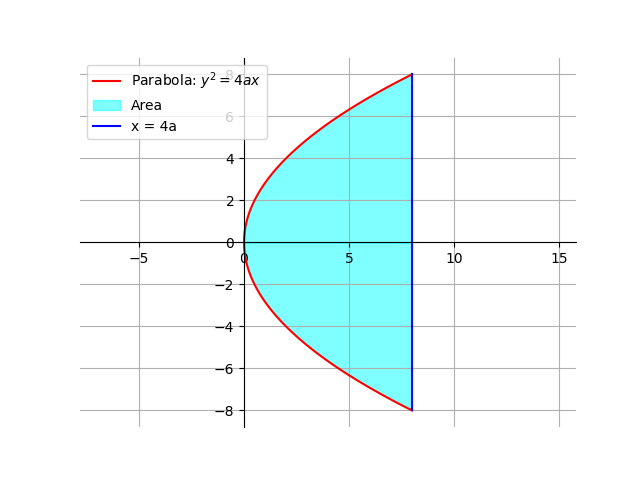
\includegraphics[width=0.6\linewidth]{figs/Figure_1.png}
	  \caption{ Area bounded by $y^2 =  4ax$ and $x=4a$ }
   \label{stemplot}
\end{figure}

The given parabola can be expressed as conics with parameters\\
\begin{align}
	\vec{V}=\myvec{
		0 & 0
   \\
	0 & 1
 }, \vec{u} = \myvec{ -2a  \\
0 } , f =0 
 \end{align}
 
 For line $ x = 4a $ the parameters are

\begin{align}
	L : \vec{x} = \vec{h} +\kappa \vec{m} ,\kappa \in R\\
	\vec{h}=\myvec{
		 4a \\	0 }, \vec{m} = \myvec{0 \\1}
 \end{align}

 To  points of intersection of line with conic section
 \begin{align}
  \vec{x_i} &= \vec{h} + \kappa_i \vec{m}
\end{align}
where 


\begin{align}
	\kappa_i = \frac{1}{\vec{{m}^{\top}Vm }}\left(-\vec{{m}^{\top}(Vh+u)} \pm \sqrt{\sbrak{\vec{m^{\top}(Vh+u)  }}^{2} - g(\vec{h})(\vec{{m}^{\top}Vm} })    \right)
\end{align}
Substituting from the above ,  we get 
\begin{align}        \kappa_i = 4a , -4a    \end{align}
yeilding the points of intersections

\begin{align}   
 \vec{x_1}= \myvec{4a\\ 4a }    , \vec{x_2}= \myvec{4a\\ -4a }   \end{align}
 
From figure the area bounded by the curve  $y^{2} = 4ax$ and line $x = 4a$ is given by 
\begin{align}
	4\sqrt{a}\ \int_{0}^{4a}  \sqrt{x} \,dx = \frac{256}{3}
\end{align}
by solving above equation the value of $a = 2 $ 

\end{document}  
\end{document}


